\documentclass[tikz,border=2pt]{standalone}
\usepackage{amsmath}
\usepackage{pgfplots}
\pgfplotsset{compat=1.18}
\usetikzlibrary{arrows.meta}
\begin{document}
% Battle of the Sexes in payoff space (v_1, v_2): the pure equilibria (O,O) = (2,1) and (F,F) = (1,2),
% the mixed equilibrium (p = 2/3, q = 1/3) with expected payoffs (2/3, 2/3), and the two mismatches
% at (0,0). Player 1 prefers (O,O), player 2 prefers (F,F); both pure equilibria lie in the shaded
% quadrant north-east of the mixed one, which they Pareto dominate.
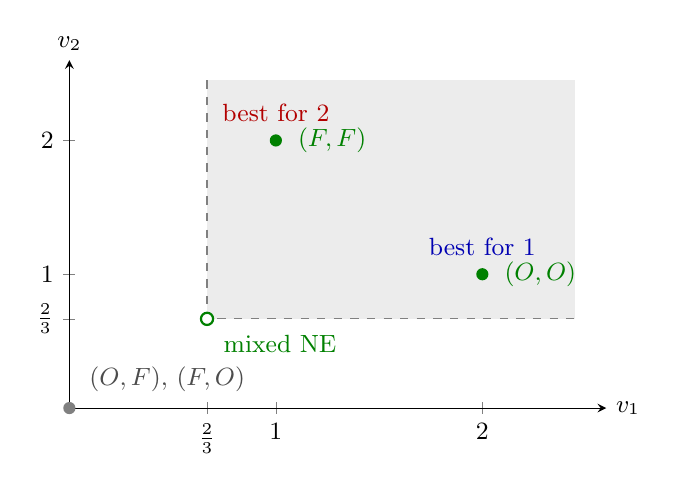
\begin{tikzpicture}[font=\small, >={Latex[length=2mm]}]
  \begin{axis}[
    axis lines=left, xmin=0, xmax=2.6, ymin=0, ymax=2.6,
    xtick={0.6667,1,2}, xticklabels={$\tfrac{2}{3}$,$1$,$2$},
    ytick={0.6667,1,2}, yticklabels={$\tfrac{2}{3}$,$1$,$2$},
    xlabel={$v_1$}, ylabel={$v_2$},
    xlabel style={anchor=west, at={(axis description cs:1.0,0.0)}},
    ylabel style={rotate=-90, anchor=south, at={(axis description cs:0,1.0)}},
    width=8.4cm, height=6cm, clip=false]
    % payoffs that Pareto dominate the mixed equilibrium
    \fill[gray!15] (axis cs:0.6667,0.6667) rectangle (axis cs:2.45,2.45);
    \draw[gray, dashed, thin] (axis cs:0.6667,2.45) -- (axis cs:0.6667,0.6667) -- (axis cs:2.45,0.6667);
    % pure equilibria
    \fill[green!50!black] (axis cs:2,1) circle (2.2pt);
    \fill[green!50!black] (axis cs:1,2) circle (2.2pt);
    \node[green!50!black, anchor=west] at (axis cs:2.06,1) {$(O,O)$};
    \node[green!50!black, anchor=west] at (axis cs:1.06,2) {$(F,F)$};
    \node[blue!70!black, anchor=south] at (axis cs:2,1.07) {best for 1};
    \node[red!70!black, anchor=south] at (axis cs:1,2.07) {best for 2};
    % mixed equilibrium
    \draw[green!50!black, thick, fill=white] (axis cs:0.6667,0.6667) circle (2.2pt);
    \node[green!50!black, anchor=north west] at (axis cs:0.7,0.62) {mixed NE};
    % mismatches
    \fill[gray] (axis cs:0,0) circle (2.2pt);
    \node[gray!60!black, anchor=south west] at (axis cs:0.05,0.05) {$(O,F)$, $(F,O)$};
  \end{axis}
\end{tikzpicture}
\end{document}
